\section*{Overfitting}

\label{sec:overfitting}

\vspace{5mm}

\newcommand{\quotes}[1]{``#1''}

\quotes{Overfitting occurs when our hypothesis fits the training data "too well"}. From Understanding Machine Learning - From Theory To Algorithms. \\

\begin{center}
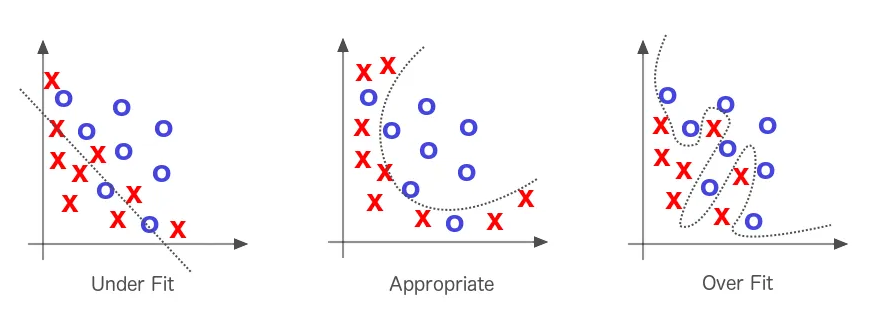
\includegraphics[scale=0.4]{overfitting.png}
\end{center}

Let $S$ be a training set sampled according to the probability distribution $\mathcal{D}$.
An algorithm $A$ overfits if the difference between the \textit{true risk} of its output $L_{\mathcal{D}}(A(S))$ and the \textit{empirical risk} of its output $L_S(A(S))$ is large. \\

\textit{Note}: Recall from the \hyperref[sec:bias-complexity-trade-off]{bias-complexity trade-off} that overfitting is also when $\epsilon_{app}$ (error made by the best predictor) is low and thus $\epsilon_{est}$ (difference between the error of the best predictor and the error of the used predictor) is high. \\

\underline{Stability} \\

An algorithm is stable if a small change in input gives a small change in output. \\

Let $S^{(i)}$ be a training set where we replace the \textit{i-th} element by $z'$: $S^{(i)}=(z_1,...,z_{i-1}, z', z_{i+1}, ... , z_m)$. We measure an effect of a small change comparing the losses $\ell(A(S^{(i)}),z_i)$ and $\ell(A(S),z_i)$ ($z_i$ is the value to predict). 

We note that the algorithm trained on $S^{(i)}$ doesn't observe $z_i$ while the algorithm trained on $S$ does. Intuitively, we should have $\ell(A(S^{(i)}),z_i) - \ell(A(S),z_i) \geq 0$. \\

$A$ is stable on average if $\mathbb{E}_{(S,z') \sim \mathcal{D}^{m+1}, i \sim U(m)}[\ell(A(S^{(i)}),z_i) - \ell(A(S),z_i)]$ is small. \\

Theorem: 

$$\mathbb{E}_{S \sim \mathcal{D}}[L_{\mathcal{D}}(A(S)) - L_S(A(S))] = \mathbb{E}_{(S,z') \sim \mathcal{D}^{m+1}, i \sim U(m)}[\ell(A(S^{(i)}),z_i) - \ell(A(S),z_i)]$$

With $U(m)$ the uniform distribution over $m$. \\

Thanks to this theorem we have the following: $A$ is a stable algorithm <=> second term is small <=> first term is small <=> $A$ does not overfit \\

\underline{Regularization} \\

In this part we show that using regularization leads to a stable algorithm. \\

Let $A$ be a regularized algorithm:

$$A(S) = \underset{\omega}{\operatorname{argmin}} (L_S(\omega) + \lambda || \omega ||^2)$$

$f_S : \omega \mapsto L_S(\omega) + \lambda || \omega ||^2$ \\

Lemma: 

- $f_S$ is $2\lambda$-strongly convex

- For any $v$: $f_S(v) - f_S(A(S)) \geq \lambda || v - A(S) ||^2$  since $A(S)$ minimizes $f_S$ \\

We have:

\begin{align*}
  f_S(v) - f_S(u) &= L_S(v) + \lambda || v ||^2 - (L_S(u) + \lambda || u ||^2) \\
            &= L_{S^{(i)}}(v) + \lambda || v ||^2 - (L_{S^{(i)}}(u) + \lambda || u ||^2) \\
	   &~~~~~~~~~~~~~+ \frac{1}{m}(\ell(v, z_i) - \ell(v, z')) - \frac{1}{m}(\ell(u, z_i) - \ell(u, z'))
\end{align*}

We removed the loss computed on the additional observation $z'$ and we added the loss computed on observation $z_i$.

\begin{align*}
  f_S(v) - f_S(u) &= L_{S^{(i)}}(v) + \lambda || v ||^2 - (L_{S^{(i)}}(u) + \lambda || u ||^2) \\
	   &~~~~~~~~~~~~~+ \frac{\ell(v, z_i) - \ell(u, z_i)}{m} + \frac{\ell(u, z') - \ell(v, z')}{m}
\end{align*}

Choosing $v = A(S^{(i)})$ and $u = A(S)$:

\begin{align*}
  f_S(A(S^{(i)})) - f_S(A(S)) &= L_{S^{(i)}}(A(S^{(i)})) + \lambda || A(S^{(i)} ||^2 - (L_{S^{(i)}}(A(S)) + \lambda || A(S) ||^2) \\
	   &~~~~~~~~~~~~~+ \frac{\ell(A(S^{(i)}), z_i) - \ell(A(S), z_i)}{m} + \frac{\ell(A(S), z') - \ell(A(S^{(i)}), z')}{m}
\end{align*}

If $A(S^{(i)})$ minimizes $L_{S^{(i)}}(\omega) + \lambda || \omega ||^2$ (optimal coefficient): \\

$L_{S^{(i)}}(A(S^{(i)})) + \lambda || A(S^{(i)} ||^2 \leq L_{S^{(i)}}(A(S)) + \lambda || A(S) ||^2$ \\

Thus, \\

$f_S(A(S^{(i)})) - f_S(A(S)) \leq \frac{\ell(A(S^{(i)}), z_i) - \ell(A(S), z_i)}{m} + \frac{\ell(A(S), z') - \ell(A(S^{(i)}), z')}{m}$ \\

Thanks to the above lemma: \\

$ \lambda || A(S^{(i)}) - A(S) ||^2 \leq \frac{\ell(A(S^{(i)}), z_i) - \ell(A(S), z_i)}{m} + \frac{\ell(A(S), z') - \ell(A(S^{(i)}), z')}{m}$ (I) \\

By definition, if $\ell(. , z_i)$ is $\rho$-Lipschitz: \\

$\ell(A(S^{(i)}), z_i) - \ell(A(S), z_i) \leq \rho || A(S^{(i)} - A(S) ||$ \\

Similarly, \\

$\ell(A(S^{(i)}), z') - \ell(A(S), z') \leq \rho || A(S^{(i)}) - A(S) ||$ \\

Plugging these two equations in (I): \\

$\lambda || A(S^{(i)}) - A(S) ||^2 \leq \frac{2 \rho || A(S^{(i)}) - A(S) ||}{m}$ \\

$|| A(S^{(i)}) - A(S) || \leq \frac{2 \rho}{\lambda m}$ \\

Using $\rho$-Lipschitz definition: \\

$\frac{1}{\rho}(\ell(A(S^{(i)}), z_i) - \ell(A(S), z_i)) \leq \frac{2 \rho}{\lambda m}$ \\

$\ell(A(S^{(i)}), z_i) - \ell(A(S), z_i) \leq \frac{2 \rho^2}{\lambda m}$ \\

Since it is true for any $S$, $z'$, $i$ we conclude:

$$\mathbb{E}_{S \sim \mathcal{D}^m}[L_{\mathcal{D}}(A(S)) - L_S(A(S))] \leq \frac{2 \rho^2}{\lambda m}$$

We have shown that a regularized algorithm is stable and thus does not overfit.

\vspace{5mm}